\section{Especificación de los requisitos del sistema}

\subsection{Requisitos de interfaces de usuario}
\label{sec:requisitos_interfaz}

La interfaz de usuario está parcialmente definida por el sistema en el que se
integrará la nueva herramienta, pero dado el volumen de datos que va a
manejar, este va a ser un aspecto muy importante. Así, en esta sección se hará
un repaso al papel de las 5 'es' de la usabilidad definidas por Whitney
Quesenbery a partir de las propuestas de Jakob Nielsen:

\begin{description}
\item [Efectividad (Effective)] Si un usuario no puede completar la tarea que
quería realizar, lo demás no importa. En el caso del proyecto en cuestión, esta
va a ser la dimensión que va a tener un mayor peso.

\item [Eficiencia (Efficient)] Se refiere a la capacidad de la interfaz de
permitir realizar una tarea de forma correcta en el menor tiempo posible. Los
usuarios del sistema va a ser, en general, personal de administración, cuando no
ingenieros cualificados, por lo que esta es otra dimensión muy importante.

\item [Inspirador / Atractivo (Engaging)] Se refiere a cómo de satisfactorio
es el uso de la interfaz, a la calidad de la interacción. Esta es una de las
características fundamentales en proyectos abiertos al público, en el que se
pretende una participación masiva; sin embargo, el proyectante no considera que
deba tener mucho peso en este caso: la experiencia debe ser buena, pero no va a
ser un foco de atención.

\item [Tolerancia a errores (Error Tolerant)] Es muy importante que la interfaz
nos ayude en el proceso de consulta, adición y modificación de elementos, con el
objetivo de minimizar los errores en primer lugar, y de corregirlos una vez que
se han cometido.

\item [Fácil de aprender (Easy to Learn)] De nuevo, el hecho de que el sistema
vaya a ser usado por muy pocas personas, permite que no sea especialmente
importante invertir tiempo en diseñar una interfaz especialmente simple, lo
cual no es trivial cuando el sistema subyacente debe ser capaz de realizar
muchas tareas distintas.
\end{description}

\begin{figure}
\centering
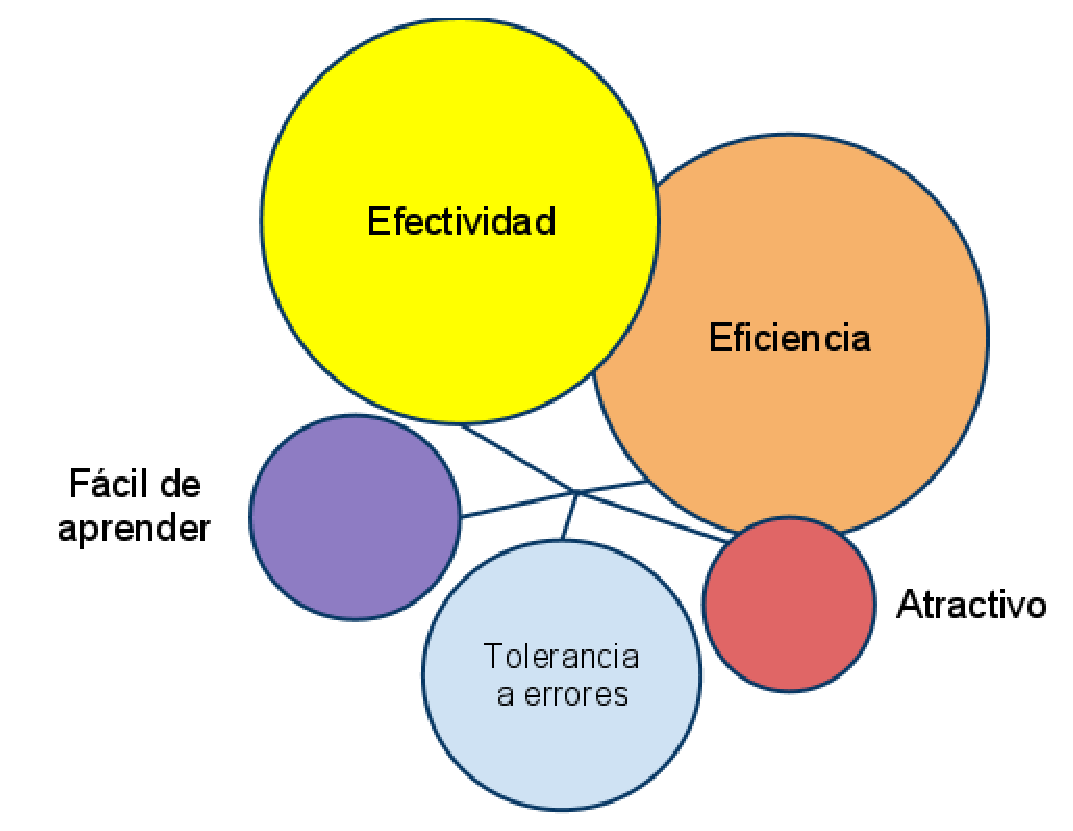
\epsfig{file=imagenes/usabilidad,width=3.5in}
\caption{Importancia de las dimensiones de usabilidad.}
\label{fig:usabilidad}
\end{figure}

\subsection{Requisitos funcionales}
\label{sec:requisitos_funcionales}

En esta sección se listan los requisitos funcionales de la aplicación agrupados
por categorías:

\subsubsection{Requisitos funcionales de la gestión de personal}
\label{sec:requisitos_personal}

\begin{itemize}
\item El usuario puede buscar y visualizar los recursos humanos y sus
registros anuales presentes en el sistema, agrupados por cliente o
individualmente, donde se puedan consultar los siguientes datos:
  \begin{itemize}
  \item Año.
  \item Salario bruto.
  \item Seguridad Social a cargo de la empresa.
  \item Horas convenio.
  \item Horas asignadas / libres.
  \item Coste / hora.
  \item Notas
  \item Fecha y autoría de la última actualización
  \end{itemize}

\item Se podrá crear un nuevo empleado mediante el registro de
sus datos. Cada
empleado tiene un número indefinido de registros anuales, donde se almacenarán
datos como salario o número de horas del convenio. Para evitar confusiones, no
puede haber dos empleados con el mismo nombre y apellidos en el sistema: en
caso de que sea necesario, se añadirá algún tipo de marca manualmente
(ejemplos: bis, padre...). Cada empleado y cada registro anual se crea con un
identificador único. Será posible, a la hora de crear registros anuales,
renovar la información del empleado: con un solo clic, se creará un registro
anual nuevo inmediatamente posterior al más reciente con los mismos datos de
salario, etc.

\item Será posible modificar los datos de cada empleado y de sus registros
anuales. Por motivos de consistencia del sistema, no será posible cambiar el
cliente al que pertenece un empleado. En caso de que se haya asignado a un
cliente que no le corresponde por error, el empleado deberá ser borrado; si el
empleado cambia de una empresa cliente a otra, será necesario crear un nuevo
empleado. Sin embargo, el sistema no sabrá que son la misma persona: consultado
el cliente de la aplicación y tutor de empresa de este proyecto, no se ha
considerado imprescindible incluir tal característica por la poca probabilidad
de que suceda. Asimismo, tampoco podrá modificarse el año de un registro anual:
de resultar sus datos incorrectos para el año actual, deberán modificarse los
datos y añadirlos en el año que les correspondiera inicialmente; si el año ha
sido introducido por error, deberá borrarse.

\item Debe ser posible eliminar empleados y registros anuales. En caso de
eliminarse un empleado, todos sus registros anuales serán borrados en
cascada, y en caso de borrar un registro anual, las horas de asignadas a ese
año también serán borradas. Debe considerarse la poca o nula utilidad de borrar
un empleado que tiene horas asignadas en el sistema, esas horas se borrarían
igualmente: aunque un empleado no formase parte finalmente en la ejecución de un
proyecto y por tanto no deban justificarse su trabajo, es interesante para
realizar estudios estadísticos ver las horas que se presentaron para ese
empleado. La peligrosidad de borrar datos de este tipo por error ha llevado al
proyectante a decidir que esta acción solamente pueda ser llevada a cabo por el
usuario administrador del sistema (ver sección \ref{sec:usuarios_del_sistema}
para obtener más información acerca de los usuarios).
\end{itemize}

\subsubsection{Requisitos funcionales de la gestión de actividades}
\label{sec:gestion_actividades}

\begin{itemize}
\item El usuario puede buscar y visualizar las actividades registradas en
el sistema, agrupadas por cliente y proyectos, donde se puedan consultar los
siguientes datos:
  \begin{itemize}
  \item Nombre de la actividad.
  \item Descripción.
  \item Fecha de inicio.
  \item Fecha de fin.
  \item Horas presentadas.
  \item Horas aprobadas.
  \item Horas justificadas.
  \end{itemize}

\item Se podrán crear nuevas actividades empleado mediante el registro de
sus datos. Para evitar confusiones, y ya que, en general, no va a tener sentido,
no puede haber dos actividades con el mismo nombre en el sistema. Cada actividad
se crea con un identificador único.

\item Será posible modificar los datos de cada actividad. Por motivos de
consistencia del sistema, no será posible cambiar el proyecto al que pertenece
una actividad. En caso de que se haya asignado a un proyecto que no le
corresponde por error, la actividad deberá ser borrada.

\item Debe ser posible eliminar actividades, excepto en el caso de que el
proyecto esté concluido. En caso de
eliminarse una actividad, todos los datos de horas asociados a ella se borrarán
en cascada. Debe considerarse la poca o nula utilidad de borrar una actividad
que tiene horas asignadas en el sistema, esas horas se borrarían igualmente:
aunque una actividad no llegase a ejecutarse finalmente en el
desarrollo de un proyecto y por tanto no deban justificarse, es
interesante para realizar estudios estadísticos ver las horas que se presentaron
para ese actividad. La peligrosidad de borrar datos de este tipo por error ha
llevado al proyectante a decidir que esta acción solamente pueda ser llevada a
cabo por el usuario administrador del sistema (ver sección
\ref{sec:usuarios_del_sistema} para obtener más información acerca de los
usuarios).
\end{itemize}

\subsubsection{Requisitos funcionales de la consulta de datos e informes}
\label{sec:requisitos_informes}

\begin{itemize}
\item Debe ser posible visualizar cuántas horas tiene asignadas un recurso en
cada uno de sus registros anuales, así como el total de horas libres (sin
asignar hasta el total de su convenio). El concepto de total de horas asignadas
no es trivial y se define como la suma de los siguientes valores:

\begin{enumerate}
  \item En los proyectos en fase de presentación, las horas presentadas aunque
sean cero, siempre que no se hayan imputado horas aprobadas o justificadas. En
el último caso, se tomarán las de la fase más avanzada.
  \item En los proyectos en fase de aprobación, las horas aprobadas aunque sean
cero, siempre que no se hayan comenzado a imputar horas justificadas.
  \item En proyectos justificados o concluidos, las horas justificadas aunque
sean cero.
\end{enumerate}

Así, el número de horas libres se define como el total menos las asignadas,
calculadas como se acaba de describir.

\item Cualquier valor de horas visible en la vista del primer punto de esta
lista debe ser un enlace a un desglose mensual por actividades que muestre los
siguientes datos:
 \begin{itemize}
  \item Nombre del empleado.
  \item Año.
  \item Mes.
  \item Proyecto.
  \item Actividad.
  \item Horas presentadas.
  \item Horas aprobadas.
  \item Horas justificadas.
  \item Horas libres.
 \end{itemize}
Ese desglose debe tener además una serie de filtros por cliente, empleado, año,
mes, proyecto y actividad para adaptarse rápidamente a las necesidades del
usuario.

\item En la vista de los proyectos y sus actividades (sección
\ref{sec:gestion_actividades}) debe haber un resumen de horas agrupadas por año
para cada empleado en la tres fases de la gestión de proyectos: presentación,
aprobación y justificación.

\item También debe haber un informe de horas agrupadas por actividad para cada
empleado en la tres fases de la gestión de proyectos: presentación,
aprobación y justificación.

\item Adicionalmente, debe existir la posibilidad de descargar una hoja de
cálculo con la información de cada empleado acerca de su participación en el
proyecto para su etapa de presentación, aprobación y justificación. La hoja de
cálculo deberá tener tantas hojas como empleados participen en el proyecto.

\item Debe existir un informe resumen global de actividades y proyectos que sea
del mismo estilo a como se venían gestionando las horas hasta ahora. Así, debe
ser del mismo estilo que la figura \ref{fig:hoja_calculo} (pág.
\pageref{fig:hoja_calculo}) y también debe ser posible descargarla como hoja de
cálculo, de modo que se conserve totalmente la funcionalidad del viejo método.
Este informe debe tener las siguientes características:
 \begin{itemize}
  \item identificar cuándo un empleado no está dado de alta en la empresa.

  \item tener en cuenta el convenio de horas del recurso para informar acerca
  de las horas que le quedan libres en un año;

  \item cuando existe un conflicto, por ejemplo, se hayan imputado más horas
  de las que deberían, el valor aparece marcado en rojo;

  \item las columnas de proyectos siguen un código de colores para indicar el
  estado en que se encuentra el proyecto: sin comenzar y presentados, azul;
aprobados, verde; justificado o concluido, naranja; denegado, rojo.

  \item cada uno de los valores, incluidos los nombres de los recursos en
  cuestión, son un enlace a otra vista donde se darán detalles acerca
  del elemento.  En esta vista, también debe mostrarse el coste/hora de
  cada empleado para calcular el coste de la selección.
 \end{itemize}

\end{itemize}


\subsubsection{Requisitos funcionales de la gestión de horas}
\label{sec:requisitos_gestion_horas}

\begin{itemize}
 \item Debe ser posible asignar horas asociadas a la vez a personal y a
actividades. Dada la división de los proyectos subvencionados en fases de
presentación, aprobación y justificación, debe poderse asignar horas de cada
uno de esos tipos. Este hecho genera algunas restricciones:
 \begin{itemize}
  \item No se pueden asignar horas presentadas a proyectos en fase de
aprobación o superior.
  \item No se pueden asignar horas aprobadas a proyectos en fase de
justificación o terminados.
  \item No se pueden asignar horas justificadas a proyectos ya terminados.
 \end{itemize}
 \item Debe ser posible asignar horas a los empleados del cliente al que
pertenece la actividad a la que se están asignando horas, y a los empleados de
clientes que figuran como cooperantes en ese proyecto. La figura de cooperante
de proyecto es previa al inicio de este proyecto.
 \item A la hora de asignar horas a una actividad, debe ser posible ver
rápidamente qué empleados tienen ya horas imputadas.
 \item Cuando una actividad se extiende durante dos o más años distintos, debe
ser inmediato elegir, si procede, a que año pertenecen las horas. Esto es muy
útil, ya que es común realizar planificaciones de forma anual,
independientemente de la duración del proyecto.
 \item En caso de que la asignación no esté \textit{preplanificada} (aunque,
en general, lo estará), debe ser posible calcular el número de horas que se
puede trabajar en un periodo basándonos en el número de horas que se dedicarán
al día y teniendo en cuenta fines de semana y otros festivos.
 \item Ya que las asignaciones se realizan, en general, por lotes, es decir,
todas las de una actividad concreta de manera consecutiva, el sistema debe
facilitar una opción del tipo \textit{asignar y seguir}, que conservaría los
datos de actividad, tipo de horas... para que se reduzca el tiempo de gestión.
 \item Dado que muchas veces se aprueban exactamente las mismas horas que se
presentaron, o se justifican las mismas que se aprobaron, debe haber una
función capaz de trasladar idénticamente las horas de un estado a otro. El
ahorro de tiempo de gestión que se produciría en estos casos es irrenunciable,
y puede llegar a ser útil incluso cuando, sin ser idénticas, las horas de un
tipo son similares a las del tipo anterior: en ese caso, solo habría que
modificar las pequeñas variaciones.
 \item La asignación de horas a un periodo se repartirá internamente por
meses (no días), de manera que las horas asignadas a un periodo que comprenda
dos meses o más se repartirán porcentualmente teniendo en cuenta el número de
días laborables de cada mes, y cuando sea posible, en múltiplos de 5. Debido a
la excesiva complejidad que se añadiría, no se tienen en cuenta las horas del
empleado en otros proyectos en el momento de la asignación.
 \item El sistema debe detectar las inconsistencias derivadas de un exceso de
horas asignadas a un empleado en un mes dado o al global del año de acuerdo a
su convenio.
 \item Debe ser posible modificar una asignación, atendiendo a las mismas
restricciones del primer punto de esta lista.
 \item Para simplificar, el concepto de borrar horas se satisface con el de
modificar asignando cero horas. De esta manera, el \textit{borrado} de horas
sigue las mismas restricciones que cualquier otra modificación.
 \item La detección de inconsistencias no debe requerir de ninguna acción del
usuario. Cualquier inconsistencia será marcada en rojo automáticamente, a la
espera de las acciones correctoras de los técnicos. Al asignar horas, el
sistema debe advertir instantáneamente de las inconsistencias producidas por
esa asignación.
\end{itemize}

\subsubsection{Requisitos funcionales de la búsqueda}

Hemos visto que el primer requisito de la gestión de recursos y de actividades
es la capacidad de buscar y visualizar la información. Para ello, cada parte
dispone de su propio filtro con funcionalidades avanzadas, por ejemplo: al
buscar personal, lo podremos hacer por nombre, cliente, año de inicio, coste
hora, ubicación o una combinación de todos; al buscar actividades, lo podremos
hacer mediante su nombre, proyecto, cliente o una combinación de todos.

Además, de acuerdo con el cliente pero a propuesta del proyectante, se
determinó que sería muy útil implementar un buscador global, característica de
la que la aplicación carecía, de manera que se pudieran encontrar clientes,
proyectos y recursos y desde allí tener acceso
a cada parte del sistema relacionada, entre ellas, los nuevos módulos de
personal y actividades.

Para dar más sentido a este buscador, este debe ser simple, accesible desde el
inicio de la sesión y a lo largo de toda ella, instantáneo, versátil,
y debe priorizar datos y dar acceso a todas las funcionalidades. Para
explicar como se logrará todo lo anterior, se presenta a continuación cada
funcionalidad brevemente detallada:

\begin{description}
\item [Simple] El buscador consistirá en una única caja de búsqueda que
devolverá los resultados (clientes, proyectos y recursos humanos) coincidentes
con la consulta del usuario. Para búsqueda avanzada, deberán emplearse los
filtros específicos de cada módulo.

\item [Accesible] El buscador se convertirá en la página de inicio de la
aplicación, y estará disponible a lo largo de toda la sesión en la barra de
menú superior.

\item [Instantáneo] Gracias al uso de AJAX, el buscador será instantáneo, de
manera que cada vez que el usuario haga clic en una letra, el resultado se
actualizará automáticamente. En combinación con la siguiente característica,
los resultados deberían ser los esperados cuando solamente se hayan tecleado
unas pocas letras del elemento buscado.

\item [Priorizar datos] En lugar de ordenar los resultados por el número de
concurrencias o por identificador, el buscador ordenará los recursos humanos
por orden alfabético. En el caso de los clientes y de los proyectos, se irá un
paso más allá para tener en cuenta el número de proyectos que tiene un cliente
y el número de expedientes que tiene un proyecto. Así, los clientes con más
proyectos y los proyectos con más expedientes se mostrarán antes. Por último,
cuando una consulta devuelva los tres tipos de datos, el orden será clientes,
recursos, proyectos.

\item [Versátil] El buscador tendrá en cuenta las características más
importantes de cada elemento. Así, no solamente buscará clientes por su nombre,
sino también por su acrónimo, teléfono, dirección, descripción... Algo similar
ocurrirá con los proyectos y los recursos, de manera que si buscamos el nombre
de un cliente, se mostrará en primer lugar ese cliente, gracias a la prioridad
de datos global descrita en el apartado anterior, y también se mostrarán sus
recursos humanos y proyectos. Se implementarán, asimismo, funciones de
paginación y la posibilidad de mostrar únicamente clientes, proyectos o
recursos.

Otra característica que se implementará de cara a la versatilidad del
buscador es la capacidad para devolver resultados incluso cuando el usuario
cometa algún error. Aunque se realizará simplemente truncando la consulta cuando
no se encuentren resultados, se espera que sea suficientemente útil.

\item [Dar acceso] La idea de esta parte es la de imitar los accesos directos
que ofrecen las principales buscadores (ver figura \ref{fig:enlaces_buscador}).
Desde un cliente, podrá accederse a proyectos, facturas, contratos, archivos y
por supuesto, personal y actividades. Desde un proyecto, podrá accederse a sus
expedientes, a sus facturas y a sus actividades.

\end{description}

\begin{figure}
\centering
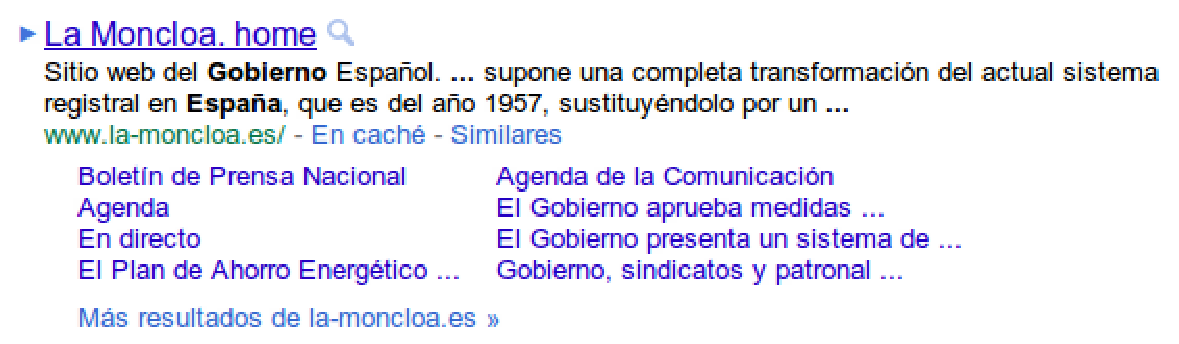
\epsfig{file=imagenes/enlaces_buscador,width=5.28in}
\caption{Enlaces de interés desde el buscador de Google.}
\label{fig:enlaces_buscador}
\end{figure}


\section{Requisitos lógicos de la base de datos}

La base de datos es uno de los componentes fundamentales de la aplicación. Se
va a hacer uso de una base de datos existente llamada \textit{ingenieria}, en la
que se integrarán las tablas necesarias para guardar todas la información
necesaria para cumplir los requisitos especificados en la sección
\ref{sec:requisitos_funcionales}. Las tablas que se añadirán son las siguientes:

\begin{description}
\item [actividad] Almacenará los datos de las actividades de cada
proyecto.

\item [coste\_personal] Contendrá la información de cada registro anual
de los empleados.

\item [personal] Guardará la información acerca de cada empleado.

\item [personal\_actividad] Guarda información básica acerca de cada asignación
realizada.

\item [personal\_horas] Almacenará los datos de horas mensuales para cada
empleado en cada actividad.
\end{description}

Los detalles sobre el diseño de la base de datos pueden consultarse en el
capítulo \ref{chp:diseno}.

\section{Casos de uso}
\label{sec:casos_de_uso}

En esta sección se especificarán los casos de uso más relevantes para cada
parte del sistema. Aunque la división física de los sistemas no es evidente, a
la hora de organizar los casos de uso se ha elegido una división lógica con
tres sistemas básicos: gestor de personal, gestor de actividades, y gestor de
horas e informes. El buscador global es tan simple que no se ha considerado
necesario elaborar un caso de uso específico.

\subsection{Gestor de personal}

\begin{figure}
\centering
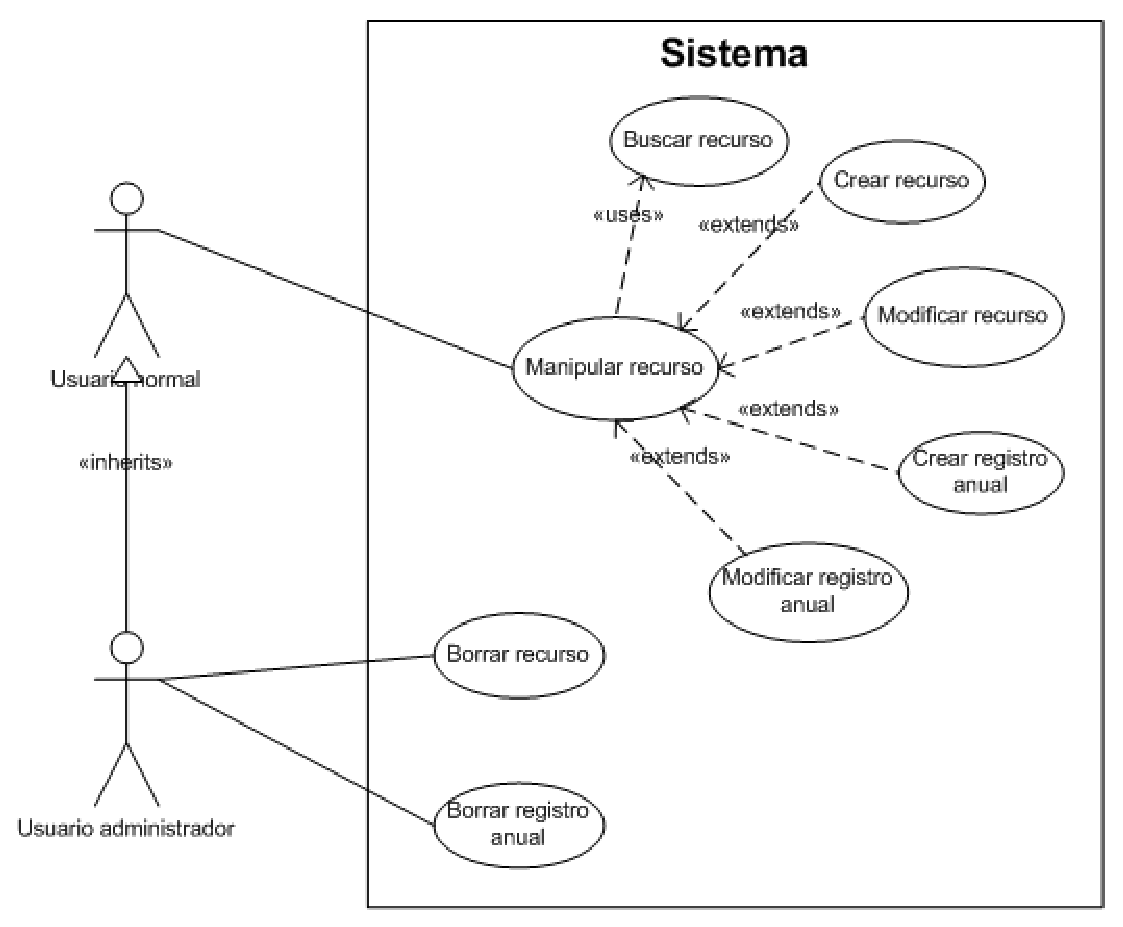
\epsfig{file=imagenes/CU_recursos,width=5.28in}
\caption{Diagrama de casos de uso para los recursos.}
\label{fig:CU_recursos}
\end{figure}

Las especificaciones que hacen referencia al gestor de personal están
descritas en la sección \ref{sec:requisitos_personal}. Todos los casos de uso
relacionados con la gestión de personal que se detallarán en este capítulo, así
como las relaciones entre los mismos, están representados en el diagrama de la
figura \ref{fig:CU_recursos}. Los usuarios del sistema y sus funciones generales
están descritos en profundidad en la sección \ref{sec:usuarios_del_sistema}.

\begin{tabular}{|p{1.25in}|p{3.65in}|}\hline
\textbf{Caso de uso} & \textbf{Buscar recurso}\\\hline\hline
\textbf{Descripción} & Búsqueda de un recurso atendiendo a diversos
parámetros\\\hline
\textbf{Actores} & Usuario normal \newline Usuario administrador\\\hline
\textbf{Precondiciones} & El usuario está autenticado en el sistema y
tiene permisos para ver el módulo de recursos\\\hline
\textbf{Pasos} &
  \begin{enumerate}
   \item El usuario introduce los datos en los campos de búsqueda.
   \item El usuario comprueba si la búsqueda es satisfactoria, y si no lo es,
vuelve al primer paso.
  \end{enumerate}
\\\hline
\textbf{Variaciones} & \\\hline
\textbf{Cuestiones} & \\\hline
\end{tabular}

\begin{tabular}{|p{1.25in}|p{3.65in}|}\hline
\textbf{Caso de uso} & \textbf{Crear recurso}\\\hline\hline
\textbf{Descripción} & Crear un nuevo recurso en el sistema. Los
atributos propios de un recurso están descritos en la sección
\ref{sec:requisitos_personal}\\\hline
\textbf{Actores} & Usuario normal \newline Usuario administrador\\\hline
\textbf{Precondiciones} & El usuario está autenticado en el sistema y
tiene permisos para ver el módulo de recursos\\\hline
\textbf{Pasos} &
  \begin{enumerate}
   \item El usuario introduce los atributos del nuevo recurso.
   \item El usuario comprueba que el recurso se ha añadido correctamente; si
no, el sistema dará un mensaje de error y el usuario debería volver al primer
paso e introducir los datos correctamente.
  \end{enumerate}
\\\hline
\textbf{Variaciones} & En cualquier momento, el usuario puede cancelar
la operación.\\\hline
\textbf{Cuestiones} & Hay una serie de campos obligatorios (nombre,
cliente...) y según los requisitos, no puede haber dos recursos
con el mismo nombre en la misma empresa.\\\hline
\end{tabular}

\begin{tabular}{|p{1.25in}|p{3.65in}|}\hline
\textbf{Caso de uso} & \textbf{Modificar recurso}\\\hline\hline
\textbf{Descripción} & Modificar los datos de un recurso en el sistema. Los
atributos propios de un recurso están descritos en la sección
\ref{sec:requisitos_personal}\\\hline
\textbf{Actores} & Usuario normal \newline Usuario administrador\\\hline
\textbf{Precondiciones} & El usuario está autenticado en el sistema y
tiene permisos para ver el módulo de recursos\newline El usuario ha
buscado el recurso usando el caso de uso «Buscar recurso»\\\hline
\textbf{Pasos} &
  \begin{enumerate}
   \item El usuario introduce los atributos actualizados del recurso.
   \item El usuario comprueba que el recurso se ha modificado correctamente; si
no, el sistema dará un mensaje de error y el usuario debería volver al primer
paso e introducir los datos correctamente.
  \end{enumerate}
\\\hline
\textbf{Variaciones} & En cualquier momento, el usuario puede cancelar
la operación.\\\hline
\textbf{Cuestiones} & Hay una serie de campos obligatorios (nombre,
cliente...) y según los requisitos, no puede haber dos recursos
con el mismo nombre en la misma empresa.\\\hline
\end{tabular}

\begin{tabular}{|p{1.25in}|p{3.65in}|}\hline
\textbf{Caso de uso} & \textbf{Crear registro anual}\\\hline\hline
\textbf{Descripción} & Crear un nuevo registro anual para un recurso del
sistema. Los atributos propios de un recurso están descritos en la sección
\ref{sec:requisitos_personal}\\\hline
\textbf{Actores} & Usuario normal \newline Usuario administrador\\\hline
\textbf{Precondiciones} & El usuario está autenticado en el sistema y
tiene permisos para ver el módulo de recursos \newline El usuario ha
buscado un recurso existente usando el caso de uso «Buscar recurso».\\\hline
\textbf{Pasos} &
  \begin{enumerate}
   \item El usuario introduce los atributos del nuevo registro anual.
   \item El usuario comprueba que el registro se ha añadido correctamente; si
no, el sistema dará un mensaje de error y el usuario debería volver al primer
paso e introducir los datos correctamente.
  \end{enumerate}
\\\hline
\textbf{Variaciones} & En cualquier momento, el usuario puede cancelar
la operación.\\\hline
\textbf{Cuestiones} & Hay una serie de campos obligatorios (año,
coste/hora...) y según los requisitos, no puede haber dos registros
anuales que hagan referencia a un mismo año.\\\hline
\end{tabular}

\begin{tabular}{|p{1.25in}|p{3.65in}|}\hline
\textbf{Caso de uso} & \textbf{Modificar registro anual}\\\hline\hline
\textbf{Descripción} & Modificar los datos de un registro anual de un recurso
del sistema. Los atributos propios de un recurso están descritos en la sección
\ref{sec:requisitos_personal}\\\hline
\textbf{Actores} & Usuario normal \newline Usuario administrador\\\hline
\textbf{Precondiciones} & El usuario está autenticado en el sistema y
tiene permisos para ver el módulo de recursos\newline El usuario ha
buscado el recurso que tiene registros anuales usando el caso de uso «Buscar
recurso»\\\hline
\textbf{Pasos} &
  \begin{enumerate}
   \item El usuario introduce los atributos actualizados del registro anual.
   \item El usuario comprueba que el recurso se ha modificado correctamente; si
no, el sistema dará un mensaje de error y el usuario debería volver al primer
paso e introducir los datos correctamente.
  \end{enumerate}
\\\hline
\textbf{Variaciones} & En cualquier momento, el usuario puede cancelar
la operación.\\\hline
\textbf{Cuestiones} & Hay una serie de campos obligatorios (año,
coste/hora...) y según los requisitos, no puede haber dos registros
anuales que hagan referencia a un mismo año.\\\hline
\end{tabular}

\begin{tabular}{|p{1.25in}|p{3.65in}|}\hline
\textbf{Caso de uso} & \textbf{Borrar recurso}\\\hline\hline
\textbf{Descripción} & Borrar los datos de un recurso en el sistema, junto con
sus registros anuales. \\\hline
\textbf{Actores} & Usuario administrador\\\hline
\textbf{Precondiciones} & El administrador ha
buscado el recurso usando el caso de uso «Buscar recurso»\\\hline
\textbf{Pasos} &
  \begin{enumerate}
   \item El administrador elige la opción de borrar recurso.
   \item El administrador confirma que desea borrar el recurso seleccionado.
   \item El administrador comprueba que el recurso se ha borrado
correctamente; si no, el sistema dará un mensaje de error.
  \end{enumerate}
\\\hline
\textbf{Variaciones} & El administrador puede cancelar la operación en lugar
de confirmarla.\\\hline
\textbf{Cuestiones} & Al borrar un recurso, se borran todas sus horas asignadas
y sus registros anuales.\\\hline
\end{tabular}

\begin{tabular}{|p{1.25in}|p{3.65in}|}\hline
\textbf{Caso de uso} & \textbf{Borrar registro anual}\\\hline\hline
\textbf{Descripción} & Borrar un registro anual de un recurso
del sistema.
\ref{sec:requisitos_personal}\\\hline
\textbf{Actores} & Usuario administrador\\\hline
\textbf{Precondiciones} & El administrador ha buscado el recurso que tiene
registros anuales usando el caso de uso «Buscar recurso»\\\hline
\textbf{Pasos} &
  \begin{enumerate}
   \item El administrador elige la opción de borrar registro anual.
   \item El administrador confirma que desea borrar el registro anual.
   \item El administrador comprueba que el registro anual se ha borrado
correctamente; sino, el sistema dará un mensaje de error.
  \end{enumerate}
\\\hline
\textbf{Variaciones} & El administrador puede cancelar la operación en lugar
de confirmarla.\\\hline
\textbf{Cuestiones} & Al borrar un registro anual, se borrarán todas las
horas asignadas a ese año.\\\hline
\end{tabular}


\subsection{Gestor de actividades}

\begin{figure}
\centering
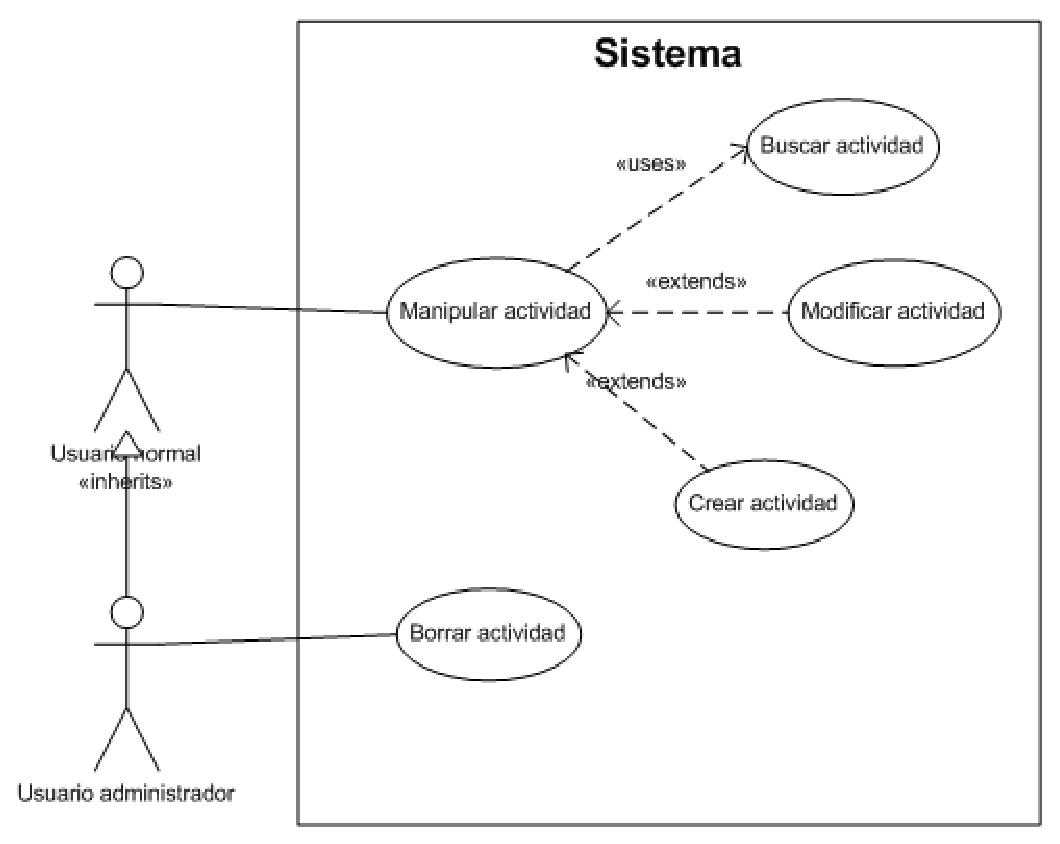
\epsfig{file=imagenes/CU_actividades,width=5in}
\caption{Diagrama de casos de uso para las actividades.}
\label{fig:CU_actividades}
\end{figure}

Las especificaciones que hacen referencia al gestor de actividades están
descritas en la sección \ref{sec:gestion_actividades}. Todos los casos de uso
relacionados con la gestión de actividades que se detallarán en este capítulo,
así como las relaciones entre los mismos, están representados en el diagrama de
la figura \ref{fig:CU_actividades}. Los usuarios del sistema y sus funciones
generales están descritos en profundidad en la sección
\ref{sec:usuarios_del_sistema}.

\begin{tabular}{|p{1.25in}|p{3.65in}|}\hline
\textbf{Caso de uso} & \textbf{Buscar actividad}\\\hline\hline
\textbf{Descripción} & Búsqueda de una actividad atendiendo a diversos
parámetros\\\hline
\textbf{Actores} & Usuario normal \newline Usuario administrador\\\hline
\textbf{Precondiciones} & El usuario está autenticado en el sistema y
tiene permisos para ver el módulo de actividades. \\\hline
\textbf{Pasos} &
  \begin{enumerate}
   \item El usuario introduce los datos en los campos de búsqueda.
   \item El usuario comprueba si la búsqueda es satisfactoria, y si no lo es,
vuelve al primer paso.
  \end{enumerate}
\\\hline
\textbf{Variaciones} & \\\hline
\textbf{Cuestiones} & \\\hline
\end{tabular}

\begin{tabular}{|p{1.25in}|p{3.65in}|}\hline
\textbf{Caso de uso} & \textbf{Crear actividad}\\\hline\hline
\textbf{Descripción} & Crear una nueva actividad en el sistema. Los
atributos propios de una actividad están descritos en la sección
\ref{sec:gestion_actividades}\\\hline
\textbf{Actores} & Usuario normal \newline Usuario administrador\\\hline
\textbf{Precondiciones} & El usuario está autenticado en el sistema y
tiene permisos para ver el módulo de actividades. El proyecto al que desea
añadir la actividad no está concluido. \\\hline
\textbf{Pasos} &
  \begin{enumerate}
   \item El usuario introduce los atributos de la nueva actividad.
   \item El usuario comprueba que la actividad se ha añadido correctamente; si
no, el sistema dará un mensaje de error y el usuario debería volver al primer
paso e introducir los datos correctamente.
  \end{enumerate}
\\\hline
\textbf{Variaciones} & En cualquier momento, el usuario puede cancelar
la operación.\\\hline
\textbf{Cuestiones} & Hay una serie de campos obligatorios (nombre,
proyecto, fechas...) y según los requisitos, no puede haber dos actividades
con el mismo nombre en un mismo proyecto.\\\hline
\end{tabular}

\begin{tabular}{|p{1.25in}|p{3.65in}|}\hline
\textbf{Caso de uso} & \textbf{Modificar actividad}\\\hline\hline
\textbf{Descripción} & Modificar los datos de una actividad en el sistema. Los
atributos propios de una actividad están descritos en la sección
\ref{sec:gestion_actividades}. \\\hline
\textbf{Actores} & Usuario normal \newline Usuario administrador\\\hline
\textbf{Precondiciones} & El usuario está autenticado en el sistema y
tiene permisos para ver el módulo de actividades. \newline El usuario ha
buscado la actividad usando el caso de uso «Buscar recurso». \newline La
actividad pertenece a un proyecto que no está concluido.\\\hline
\textbf{Pasos} &
  \begin{enumerate}
   \item El usuario introduce los atributos actualizados de la actividad.
   \item El usuario comprueba que la actividad se ha modificado correctamente;
si no, el sistema dará un mensaje de error y el usuario debería volver al primer
paso e introducir los datos correctamente.
  \end{enumerate}
\\\hline
\textbf{Variaciones} & En cualquier momento, el usuario puede cancelar
la operación.\\\hline
\textbf{Cuestiones} & Hay una serie de campos obligatorios (nombre,
proyecto, fechas...) y según los requisitos, no puede haber dos actividades
con el mismo nombre en el mismo proyecto.\\\hline
\end{tabular}

\begin{tabular}{|p{1.25in}|p{3.65in}|}\hline
\textbf{Caso de uso} & \textbf{Borrar actividad}\\\hline\hline
\textbf{Descripción} & Borrar los datos de una actividad en el sistema. \\\hline
\textbf{Actores} & Usuario administrador\\\hline
\textbf{Precondiciones} & El administrador ha
buscado la actividad usando el caso de uso «Buscar actividad».\\\hline
\textbf{Pasos} &
  \begin{enumerate}
   \item El administrador elige la opción de borrar actividad.
   \item El administrador confirma que desea borrar la actividad seleccionada.
   \item El administrador comprueba que la actividad se ha borrado
correctamente; si no, el sistema dará un mensaje de error.
  \end{enumerate}
\\\hline
\textbf{Variaciones} & El administrador puede cancelar la operación en lugar
de confirmarla.\\\hline
\textbf{Cuestiones} & Al borrar una actividad, se borran todas sus horas
asignadas a cualquier recurso.\\\hline
\end{tabular}

\subsection{Gestor de horas e informes}

\begin{figure}
\centering
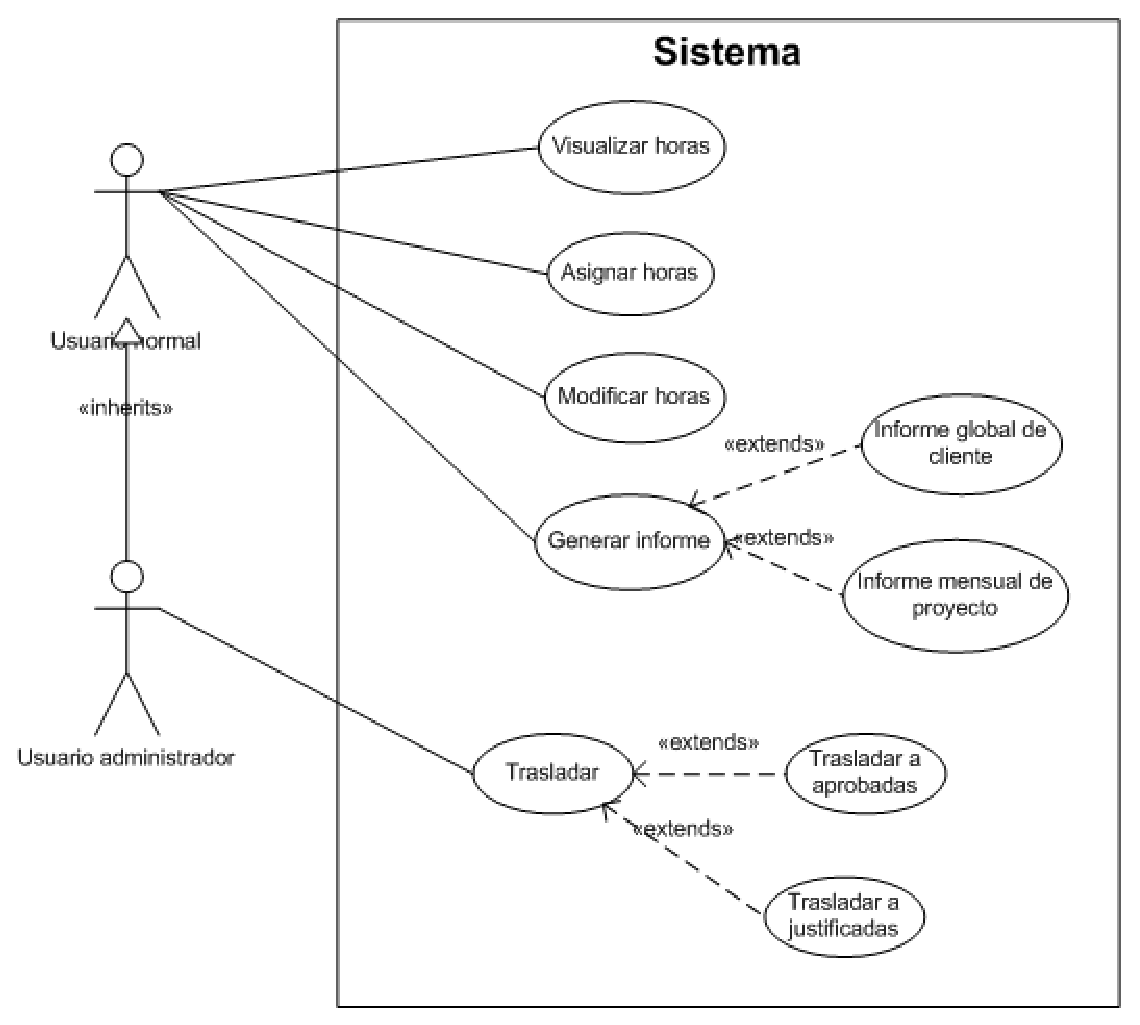
\epsfig{file=imagenes/CU_horas,width=5.28in}
\caption{Diagrama de casos de uso para las gestión de horas.}
\label{fig:CU_horas}
\end{figure}

Las especificaciones que hacen referencia a la gestión de horas están
descritas en la sección \ref{sec:requisitos_gestion_horas}. Todos los casos de
uso relacionados con la gestión de horas que se detallarán en este
capítulo, así como las relaciones entre los mismos, están representados en el
diagrama de la figura \ref{fig:CU_horas}. Los usuarios del sistema y sus
funciones generales están descritos en profundidad en la sección
\ref{sec:usuarios_del_sistema}.

\begin{tabular}{|p{1.25in}|p{3.65in}|}\hline
\textbf{Caso de uso} & \textbf{Visualizar detalle de horas}\\\hline\hline
\textbf{Descripción} & Visualizar las horas asociadas a actividades o recursos,
según una serie de parámetros. \\\hline
\textbf{Actores} & Usuario normal \newline Usuario administrador\\\hline
\textbf{Precondiciones} & El usuario está autenticado en el sistema y
tiene permisos para ver los módulos de actividades o recursos.\\\hline
\textbf{Pasos} &
  \begin{enumerate}
   \item El usuario pincha sobre el valor de horas que desea visualizar en
cualquier sitio dentro de los módulos de recursos o actividades.
  \end{enumerate}
\\\hline
\textbf{Variaciones} & Si el usuario no quiere ver el detalle de horas,
basta con buscar los recursos o las actividades para obtener información
básica usando los casos de uso «Buscar recurso» y «Buscar actividad».\\\hline
\textbf{Cuestiones} & Este caso de uso dirige al usuario a una nueva
ventana de su navegador.\\\hline
\end{tabular}

\begin{tabular}{|p{1.25in}|p{3.65in}|}\hline
\textbf{Caso de uso} & \textbf{Asignar horas}\\\hline\hline
\textbf{Descripción} & Asignar un número determinado de horas a un recurso en
una actividad. \\\hline
\textbf{Actores} & Usuario normal | Usuario administrador\\\hline
\textbf{Precondiciones} & El usuario está autenticado en el sistema y
tiene permisos para ver los módulos de actividades o recursos. El
recurso tiene registros anuales para el periodo que dura la actividad,
que debe pertenecer a un proyecto no concluido.\\\hline
\textbf{Pasos} &
  \begin{enumerate}
   \item El usuario selecciona la opción asignar horas en la actividad deseada.
   \item El usuario elige el recurso al que se van a asignar las horas, el
tipo de horas (con restricciones según el estado del proyecto) y el rango de
fechas en el que se distribuirán las horas.
   \item El usuario confirma que las horas se han asignado correctamente; si
no, el sistema dará un mensaje de error y el usuario deberá volver al primer
punto de esta lista.
  \end{enumerate}
\\\hline
\textbf{Variaciones} & El usuario puede cancelar la operación en
cualquier momento. Si se genera alguna inconsistencia, el sistema advierte al
usuario y enlaza al detalle de horas de la asignación.\\\hline
\textbf{Cuestiones} & La asignación se realiza, cuando es posible, por
bloques de 5 horas. Una asignación puede sobrescribir otra asignación
anterior. \\\hline
\end{tabular}

\begin{tabular}{|p{1.25in}|p{3.65in}|}\hline
\textbf{Caso de uso} & \textbf{Modificar horas}\\\hline\hline
\textbf{Descripción} & Modificar una asignación de horas a nivel de mes.
\\\hline
\textbf{Actores} & Usuario normal \newline Usuario administrador\\\hline
\textbf{Precondiciones} & El usuario está autenticado en el sistema y
tiene permisos para ver los módulos de actividades o recursos. Las horas
asignadas son modificables según las restricciones por el estado del
proyecto. \\\hline
\textbf{Pasos} &
  \begin{enumerate}
   \item El usuario pincha sobre las horas que desea modificar en el detalle
mensual de horas.
   \item El usuario introduce el nuevo valor y confirma la operación.
  \end{enumerate}
\\\hline
\textbf{Variaciones} & El usuario puede cancelar la operación en
cualquier momento.\\\hline
\textbf{Cuestiones} & Una modificación de este tipo modifica la suma
global de horas asignadas, es decir, la diferencia con las horas previas
no se sustrae o se añade en otro mes.\\\hline
\end{tabular}

\begin{tabular}{|p{1.25in}|p{3.65in}|}\hline
\textbf{Caso de uso} & \textbf{Generar informe global de cliente}\\\hline\hline
\textbf{Descripción} & Genera una hoja de cálculo con el estado actual de la
base de datos resumiendo la asignación de horas para todos los empleados del
cliente en todos los proyectos.
\\\hline
\textbf{Actores} & Usuario normal \newline Usuario administrador\\\hline
\textbf{Precondiciones} & El usuario está autenticado en el sistema y
tiene permisos para ver los módulos de actividades o recursos. \\\hline
\textbf{Pasos} &
  \begin{enumerate}
   \item El usuario pincha sobre el enlace de generación de la hoja de cálculo.
   \item El usuario abre o guarda el archivo (el comportamiento varía según el
navegador empleado).
  \end{enumerate}
\\\hline
\textbf{Variaciones} & \\\hline
\textbf{Cuestiones} & La generación puede llevar varios segundos
dependiendo de la cantidad de datos a exportar.\\\hline
\end{tabular}

\begin{tabular}{|p{1.25in}|p{3.65in}|}\hline
\textbf{Caso de uso} & \textbf{Generar informe mensual de
proyecto}\\\hline\hline
\textbf{Descripción} & Genera una hoja de cálculo con el estado actual de la
base de datos resumiendo la asignación de horas por mes para todos los empleados
del cliente en todos los proyectos. Cada empleado tiene su propia hoja en el
archivo.
\\\hline
\textbf{Actores} & Usuario normal \newline Usuario administrador\\\hline
\textbf{Precondiciones} & El usuario está autenticado en el sistema y
tiene permisos para ver los módulos de actividades o recursos. \\\hline
\textbf{Pasos} &
  \begin{enumerate}
   \item El usuario pincha sobre el enlace de generación de la hoja de cálculo
adecuado: presentación, aprobación o justificación.
   \item El usuario abre o guarda el archivo (el comportamiento varía según el
navegador empleado).
  \end{enumerate}
\\\hline
\textbf{Variaciones} & \\\hline
\textbf{Cuestiones} & La generación puede llevar varios segundos
dependiendo de la cantidad de datos a exportar.\\\hline
\end{tabular}

\begin{tabular}{|p{1.25in}|p{3.65in}|}\hline
\textbf{Caso de uso} & \textbf{Trasladar horas}\\\hline\hline
\textbf{Descripción} & Traslada todas las horas presentadas a aprobadas, o
todas las aprobadas a justificadas, para un proyecto concreto, y lo hace
actividad por actividad y empleado por empleado.
\\\hline
\textbf{Actores} & Usuario administrador\\\hline
\textbf{Precondiciones} & El administrador ha
buscado la actividad usando el caso de uso «Buscar actividad». \\\hline
\textbf{Pasos} &
  \begin{enumerate}
   \item El administrador pincha sobre el enlace de traslación de horas
adecuado.
   \item El administrador confirma la operación y comprueba que las horas se han
trasladado correctamente.
  \end{enumerate}
\\\hline
\textbf{Variaciones} & El administrador puede cancelar la operación en
lugar de confirmarla. \\\hline
\textbf{Cuestiones} & La traslación conserva todas las horas, incluso
si generan inconsistencias.\\\hline
\end{tabular}

\newpage
\section{Protección de datos}

Ingeniería e Innovación necesita poseer datos sensibles de sus clientes y
de los empleados de estos para llevar a cabo su actividad. Por ello, en los
contratos que firma con sus clientes, se siguen escrupulosamente las pautas
marcadas por la Ley Orgánica 15/1999 de 13 de diciembre de Protección de Datos
de Carácter Personal (LOPD). Así, los clientes son previamente
informados de modo expreso, preciso e inequívoco:

\begin{itemize}
\item[1)] de la existencia de un fichero o tratamiento de datos de carácter
personal, de la finalidad de la recogida de éstos y de los destinatarios de la
información;

\item[2)] del carácter obligatorio o facultativo de su respuesta a las preguntas
que les sean planteadas;

\item[3)] de las consecuencias de la obtención de los datos o de la negativa a
suministrarlos;

\item[4)] de la posibilidad de ejercitar los derechos de acceso, rectificación,
cancelación y oposición;

\item[5)] de la identidad y dirección del responsable del tratamiento o, en su
caso, de su representante.
\end{itemize}



